\documentclass[../main.tex]{subfiles}
\begin{document}
\subsection{Гистограммы и графики плотности распределения}
	\begin{figure}[H]
		\centering
		\begin{tabular}{ccc}
			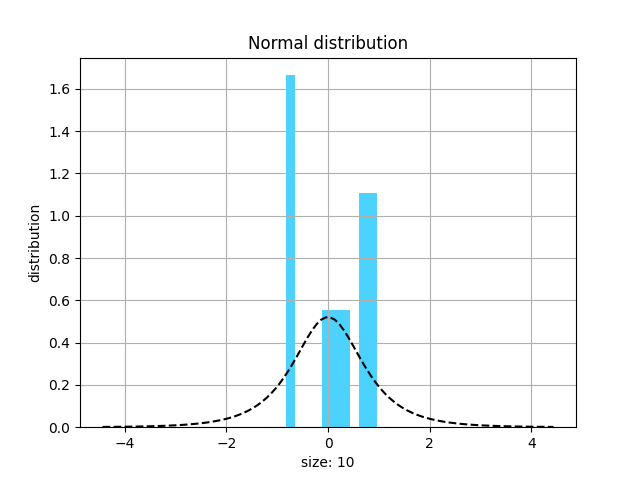
\includegraphics[width=55mm, height =0.25\textheight]{figures/NormalNumber10.png} 
			&
			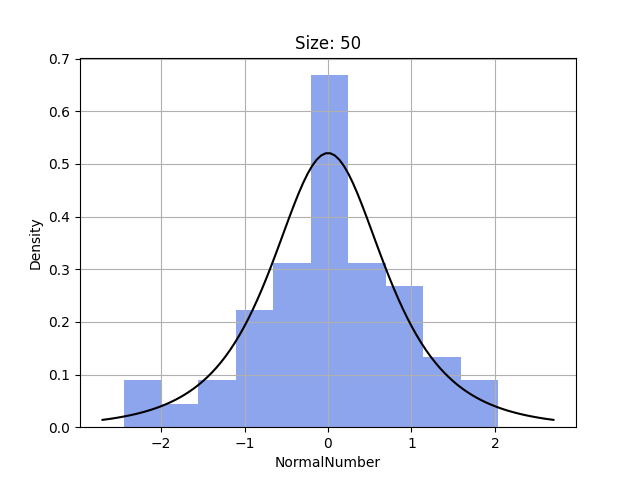
\includegraphics[width=55mm, height =0.25\textheight]{figures/NormalNumber50.png}
			&
			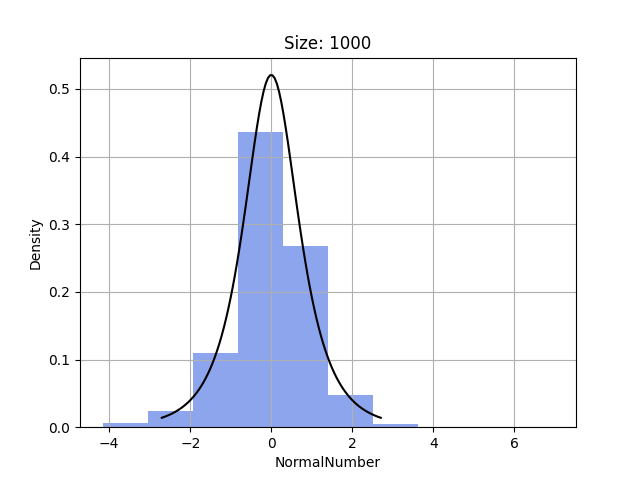
\includegraphics[width=55mm, height =0.25\textheight]{figures/NormalNumber1000.png}
		\end{tabular}
		\caption{Нормальное распределение} 
		\label{fig:normal}
	\end{figure}
	
	\begin{figure}[H]
		\centering
		\begin{tabular}{ccc}
			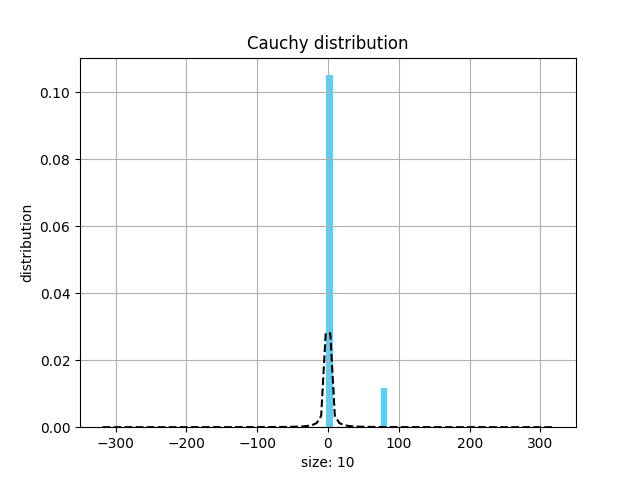
\includegraphics[width=55mm, height =0.25\textheight]{figures/CauchyNumber10.png} 
			&
			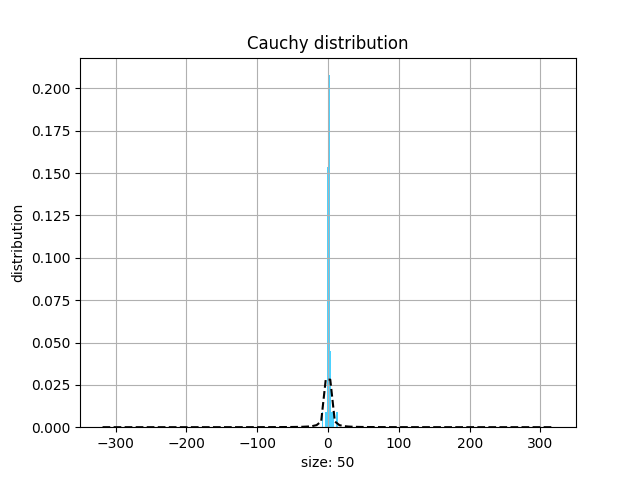
\includegraphics[width=55mm, height =0.25\textheight]{figures/CauchyNumber50.png}
			&
			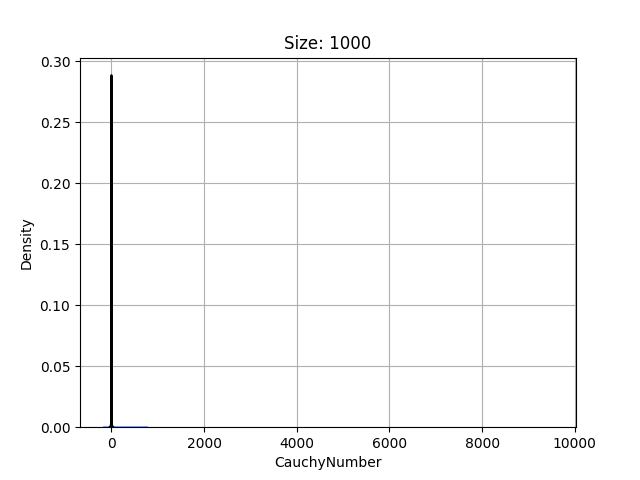
\includegraphics[width=55mm, height =0.25\textheight]{figures/CauchyNumber1000.png}
		\end{tabular}
		\caption{Распределение Коши} 
		\label{fig:normal}
	\end{figure}
	
	\begin{figure}[H]
		\centering
		\begin{tabular}{ccc}
			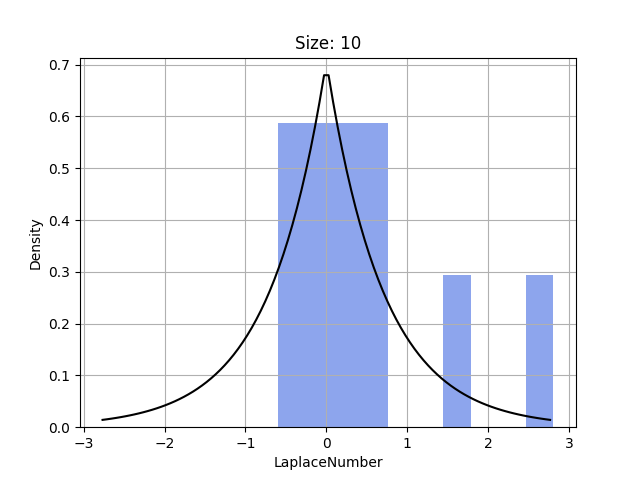
\includegraphics[width=55mm, height =0.25\textheight]{figures/LaplaceNumber10.png} 
			&
			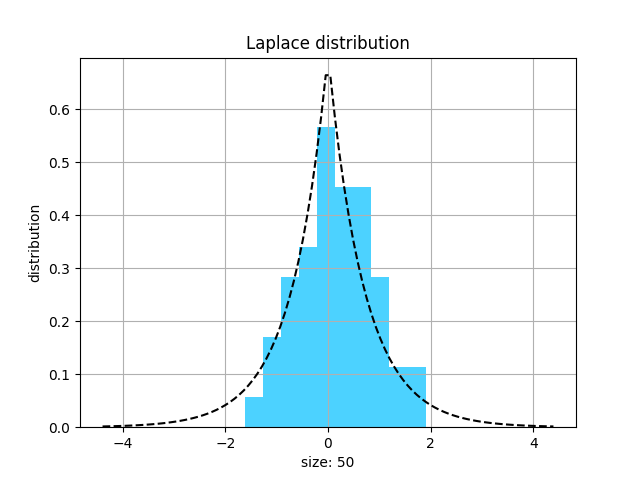
\includegraphics[width=55mm, height =0.25\textheight]{figures/LaplaceNumber50.png}
			&
			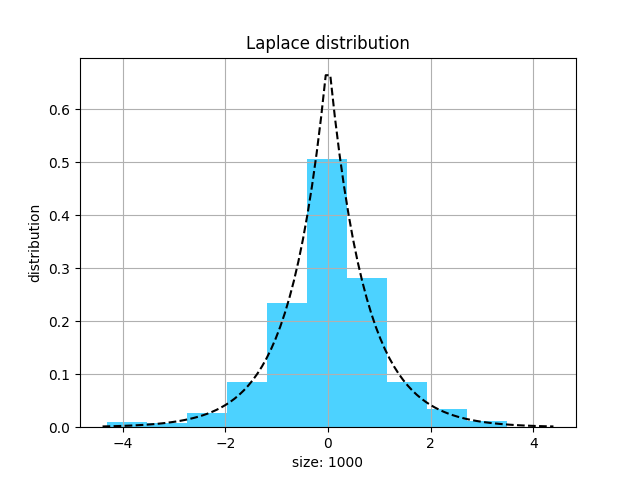
\includegraphics[width=55mm, height =0.25\textheight]{figures/LaplaceNumber1000.png}
		\end{tabular}
		\caption{Распределение Лапласа} 
		\label{fig:normal}
	\end{figure}
	
	\begin{figure}[H]
		\centering
		\begin{tabular}{ccc}
			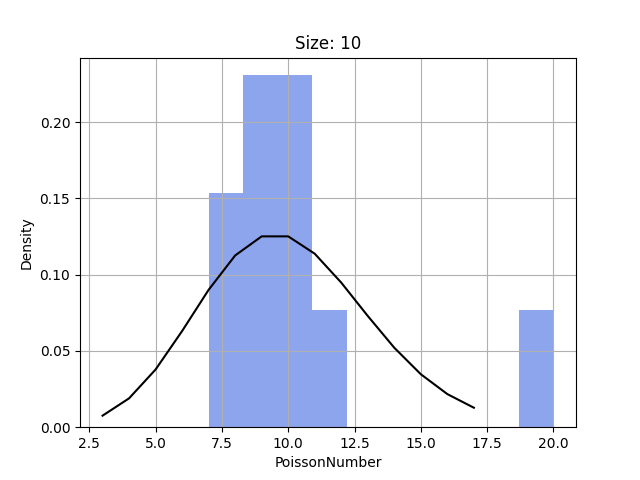
\includegraphics[width=55mm, height =0.25\textheight]{figures/PoissonNumber10.png} 
			&
			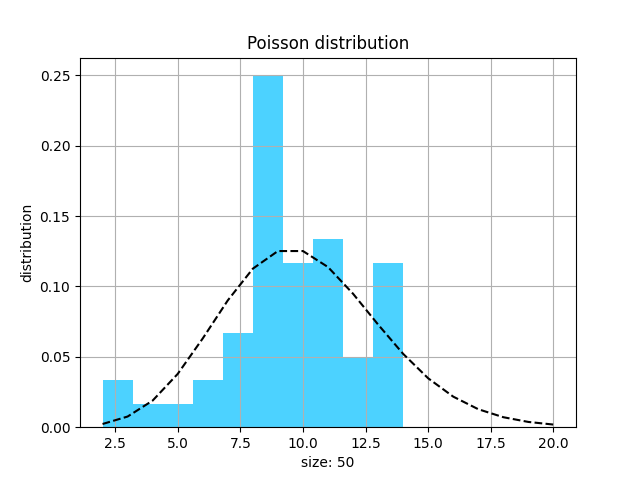
\includegraphics[width=55mm, height =0.25\textheight]{figures/PoissonNumber50.png}
			&
			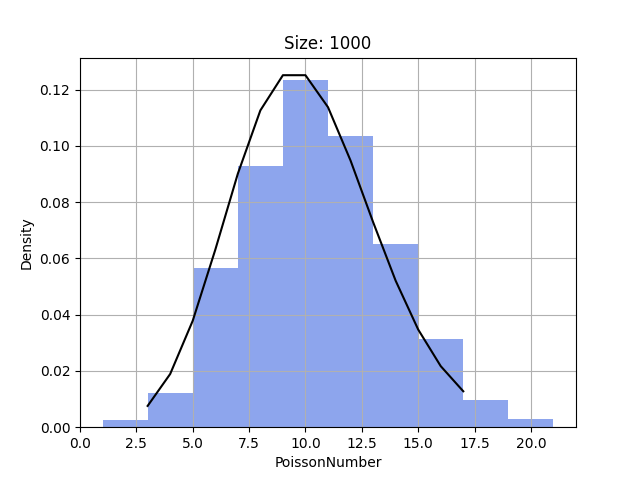
\includegraphics[width=55mm, height =0.25\textheight]{figures/PoissonNumber1000.png}
		\end{tabular}
		\caption{Распределение Пауссона} 
		\label{fig:normal}
	\end{figure}
	
	\begin{figure}[H]
		\centering
		\begin{tabular}{ccc}
			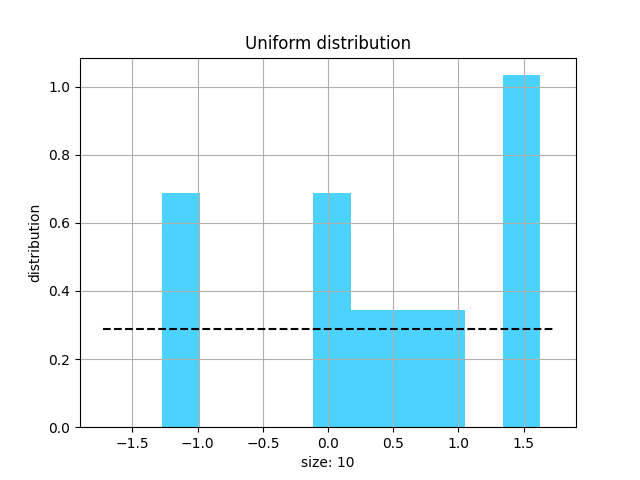
\includegraphics[width=55mm, height =0.25\textheight]{figures/UniformNumber10.png} 
			&
			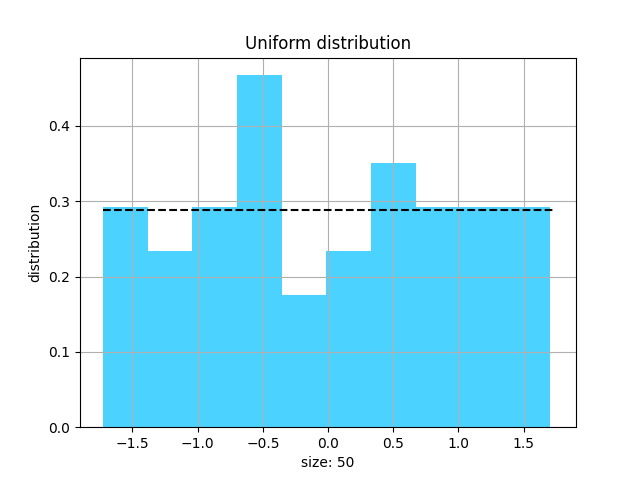
\includegraphics[width=55mm, height =0.25\textheight]{figures/UniformNumber50.png}
			&
			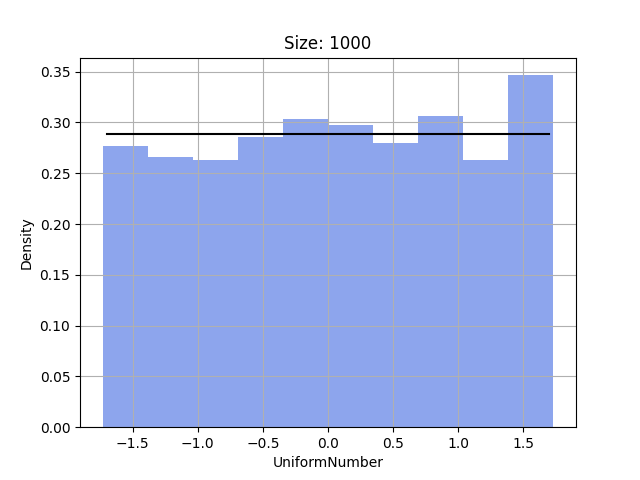
\includegraphics[width=55mm, height =0.25\textheight]{figures/UniformNumber1000.png}
		\end{tabular}
		\caption{Равномерное распределение} 
		\label{fig:normal}
	\end{figure}
	
	\subsection{Характеристики положения и рассеяния}
	
	\begin{table}[H]
    \centering
    \begin{tabular}{|l||c|c|c|c|c|}
        \hline
        & $\overline{x}$ & $med x$ & $z_R$ & $z_Q$ & $z_{tr}$\\\hline\hline
        n=10 & & & & &\\\hline
        $E(z)$ & 0.00783 & 0.000649 & 0.011704 & 0.316865 & 0.279662\\\hline
        $D(z)$ & 0.101986 & 0.138258 & 0.182348 & 0.130745 & 0.118405\\\hline
        E(z) \pm \sqrt{D(z)} & [0.3272; & [0.3725; & [0.4387; & [-0.6785; & [0.6238; \\
		&  -0.3115] &  -0.3712] & -0.4153] & -0.0447] & -0.0644] \\\hline
		\widehat{E}(z) & 0 & 0 & 0 & 0 & 0\\\hline
        n=100 & & & & &\\\hline
        $E(z)$ & 0.003355 & 0.005395 & -0.002108 & 0.018576 & 0.032072\\\hline
        $D(z)$ & 0.009793 & 0.014229 & 0.090936 & 0.012374 & 0.011337\\\hline
        E(z) \pm \sqrt{D(z)} & [0.1023; & [0.1247; & [0.2994; & [0.1298; & [0.1385; \\
		&  -0.0956] &  -0.1139] & -0.3037] & -0.0927] & -0.0744] \\\hline
		\widehat{E}(z) & 0 & 0 & 0 & 0 & 0\\\hline
        n=1000 & & & & &\\\hline
        $E(z)$ & -0.000548 & -0.000252 & -0.000612 & 0.001267 & 0.002887\\\hline
        $D(z)$ & 0.000986 & 0.001567 & 0.061974 & 0.001201 & 0.00119\\\hline
        E(z) \pm \sqrt{D(z)} & [0.0309; & [0.0393; & [0.2483; & [0.0359; & [0.0374; \\
		&  -0.0319] &  -0.0398] & -0.2496] & -0.0334] & -0.0316] \\\hline
		\widehat{E}(z) & 0 & 0 & 0 & 0 & 0\\\hline
    \end{tabular}
    \caption{Нормальное распределение}
    \label{tab:normal}
    \end{table}
    
    \begin{table}[H]
    \centering
    \begin{tabular}{|l||c|c|c|c|c|}
        \hline
        & $\overline{x}$ & $med x$ & $z_R$ & $z_Q$ & $z_{tr}$\\\hline\hline
        n=10 & & & & &\\\hline
        $E(z)$ & 0.28875 & -0.005228 & 1.474197 & 1.273873 & 0.737032\\\hline
        $D(z)$ & 93.628602 & 0.336607 & 2187.372982 & 15.339821 & 2.373734\\\hline
        E(z) \pm \sqrt{D(z)} & [9.9649; & [0.5750; & [48.2436; & [5.1905; & [2.2777; \\
		&  -9.3874] &  -0.5854] & -45.2952] & -2.6427] & -0.8037] \\\hline
		\widehat{E}(z) & - & 0 & - & 0 & 0\\\hline
        n=100 & & & & &\\\hline
        $E(z)$ & -1.271446 & -0.007581 & -62.483751 & 0.016789 & 0.030006\\\hline
        $D(z)$ & 612.101245 & 0.02479 & 1508295.961798 & 0.053915 & 0.027198\\\hline
        E(z) \pm \sqrt{D(z)} & [23.4692; & [0.1498; & [1165.6432; & [0.2489; & [0.1949; \\
		&  -26.0121] &  -0.1650] & -1290.6107] & -0.2154] & -0.1349] \\\hline
		\widehat{E}(z) & - & 0 & - & 0 & 0\\\hline
        n=1000 & & & & &\\\hline
        $E(z)$ & 2.811126 & 0.001284 & 1382.966803 & 0.004563 & 0.005812\\\hline
        $D(z)$ & 3054.863093 & 0.002503 & 761373096.375691 & 0.005074 & 0.002654\\\hline
        E(z) \pm \sqrt{D(z)} & [58.0819; & [0.0513; & [28975.9567; & [0.0757; & [0.0573; \\
		&  -52.4596] &  -0.0487] & -26210.0231] & -0.0666] & -0.0457] \\\hline
		\widehat{E}(z) & - & 0 & - & 0 & 0\\\hline
    \end{tabular}
    \caption{Распределение Коши}
    \label{tab:normal}
    \end{table}
    
    \begin{table}[H]
    \centering
    \begin{tabular}{|l||c|c|c|c|c|}
        \hline
        & $\overline{x}$ & $med x$ & $z_R$ & $z_Q$ & $z_{tr}$\\\hline\hline
        n=10 & & & & &\\\hline
        $E(z)$ & 0.009953 & 0.006635 & 0.010806 & 0.312161 & 0.246866\\\hline
        $D(z)$ & 0.098919 & 0.07654 & 0.406287 & 0.117389 & 0.082069\\\hline
        E(z) \pm \sqrt{D(z)} & [0.3245; & [0.2833; & [0.6482; & [0.6548; & [0.5333; \\
		&  -0.3046] &  -0.2700] & -0.6266] & -0.0305] & -0.0396] \\\hline
		\widehat{E}(z) & 0 & 0 & 0 & 0 & 0\\\hline
        n=100 & & & & &\\\hline
        $E(z)$ & 0.003592 & 0.001682 & 0.012879 & 0.018669 & 0.022897\\\hline
        $D(z)$ & 0.010065 & 0.00539 & 0.439571 & 0.009504 & 0.005988\\\hline
        E(z) \pm \sqrt{D(z)} & [0.1039; & [0.0751; & [0.6759; & [0.1162; & [0.1003; \\
		&  -0.0967] &  -0.0717] & -0.6501] & -0.0788] & -0.0545] \\\hline
		\widehat{E}(z) & 0 & 0 & 0 & 0 & 0\\\hline
        n=1000 & & & & &\\\hline
        $E(z)$ & 0.001955 & 0.000966 & 0.016544 & 0.004052 & 0.003654\\\hline
        $D(z)$ & 0.00102 & 0.000499 & 0.424402 & 0.001079 & 0.000609\\\hline
        E(z) \pm \sqrt{D(z)} & [0.0339; & [0.0233; & [0.6680; & [0.0369; & [0.0283; \\
		&  -0.0300] &  -0.0214] & -0.6349] & -0.0288] & -0.0210] \\\hline
		\widehat{E}(z) & 0 & 0 & 0 & 0 & 0\\\hline
    \end{tabular}
    \caption{Распределение Лапласа}
    \label{tab:normal}
    \end{table}
	
	\begin{table}[H]
    \centering
    \begin{tabular}{|l||c|c|c|c|c|}
        \hline
        & $\overline{x}$ & $med x$ & $z_R$ & $z_Q$ & $z_{tr}$\\\hline\hline
        n=10 & & & & &\\\hline
        $E(z)$ & 9.9483 & 9.8055 & 10.2655 & 10.8815 & 10.7075\\\hline
        $D(z)$ & 0.903857 & 1.31842 & 1.86576 & 1.240708 & 1.10986\\\hline
        E(z) \pm \sqrt{D(z)} & [10.8990; & [10.9537; & [11.6314; & [11.9954; & [11.7610; \\
		&  8.9976] &  8.6573] & 8.8996] & 9.7676] & 9.6540] \\\hline
		\widehat{E}(z) & 10^{+1}_{-1} & 10^{+1}_{-1} & 10^{+2}_{-2} & 10^{+2}_{-2} & 10^{+1}_{-1}\\\hline
        n=100 & & & & &\\\hline
        $E(z)$ & 9.98972 & 9.836 & 10.947 & 9.9465 & 9.93686\\\hline
        $D(z)$ & 0.107242 & 0.224604 & 1.044691 & 0.167388 & 0.131238\\\hline
        E(z) \pm \sqrt{D(z)} & [10.3172; & [10.3099; & [11.9691; & [10.3556; & [10.2991; \\
		&  9.6622] &  9.3621] & 9.9249] & 9.5374] & 9.5746] \\\hline
		\widehat{E}(z) & 10^{+1}_{-1} & 10^{+1}_{-1} & 10^{+2}_{-2} & 10^{+2}_{-2} & 10^{+1}_{-1}\\\hline
        n=1000 & & & & &\\\hline
        $E(z)$ & 10.003314 & 9.9945 & 11.662 & 9.995 & 9.867934\\\hline
        $D(z)$ & 0.009953 & 0.00522 & 0.655256 & 0.002475 & 0.011043\\\hline
        E(z) \pm \sqrt{D(z)} & [10.1031; & [10.3099; & [10.0667; & [12.4715; & [10.0447; \\
		&  9.9035] &  9.9223] & 10.8525] & 9.9453] & 9.7628] \\\hline
		\widehat{E}(z) & 10^{+1}_{-1} & 10^{+1}_{-1} & 10^{+2}_{-2} & 10^{+2}_{-2} & 10^{+1}_{-1}\\\hline
    \end{tabular}
    \caption{Распределение Пуасона}
    \label{tab:normal}
    \end{table}
    
    \begin{table}[H]
    \centering
    \begin{tabular}{|l||c|c|c|c|c|}
        \hline
        & $\overline{x}$ & $med x$ & $z_R$ & $z_Q$ & $z_{tr}$\\\hline\hline
        n=10 & & & & &\\\hline
        $E(z)$ & -0.002391 & -0.015133 & 0.003609 & 0.319112 & 0.310035\\\hline
        $D(z)$ & 0.107682 & 0.245241 & 0.044913 & 0.133545 & 0.165372\\\hline
        E(z) \pm \sqrt{D(z)} & [0.3258; & [0.4801; & [0.2155; & [0.6846; & [0.7167; \\
		&  -0.3305] &  -0.5104] & -0.2083] & -0.0463] & -0.0966] \\\hline
		\widehat{E}(z) & 0 & 0 & 0 & 0 & 0\\\hline
        n=100 & & & & &\\\hline
        $E(z)$ & -0.001485 & -0.002167 & 0.001143 & 0.012677 & 0.0321\\\hline
        $D(z)$ & 0.010127 & 0.02873 & 0.000586 & 0.015531 & 0.019983\\\hline
        E(z) \pm \sqrt{D(z)} & [0.0991; & [0.1673; & [0.0254; & [0.1373; & [0.1735; \\
		&  -0.1021] &  -0.1717] & -0.0231] & -0.1119] & -0.1093] \\\hline
		\widehat{E}(z) & 0 & 0 & 0 & 0 & 0\\\hline
        n=1000 & & & & &\\\hline
        $E(z)$ & 0.001444 & 0.001939 & 1.5e-05 & 0.003171 & 0.005647\\\hline
        $D(z)$ & 0.001067 & 0.003119 & 6e-06 & 0.001656 & 0.002112\\\hline
        E(z) \pm \sqrt{D(z)} & [0.0341; & [0.0578; & [0.0025; & [0.0439; & [0.0516; \\
		&  -0.0312] &  -0.0539] & -0.0024] & -0.0375] & -0.0403] \\\hline
		\widehat{E}(z) & 0 & 0 & 0 & 0 & 0\\\hline
    \end{tabular}
    \caption{Нормальное распределение}
    \label{tab:normal}
    \end{table}
	
	\subsection{Боксплот Тьюки}
	
	\begin{figure}[H]
        \centering
        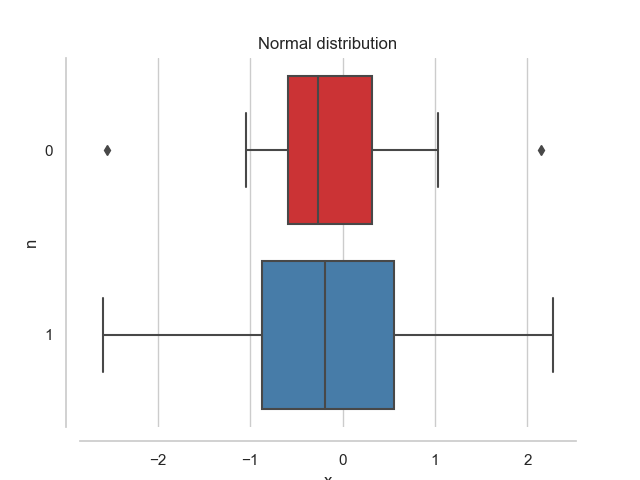
\includegraphics[scale=0.8]{figures/NormalBoxplot.png}
        \caption{Нормальное распределение}
        \label{fig:normal}
    \end{figure}
    
    \begin{figure}[H]
        \centering
        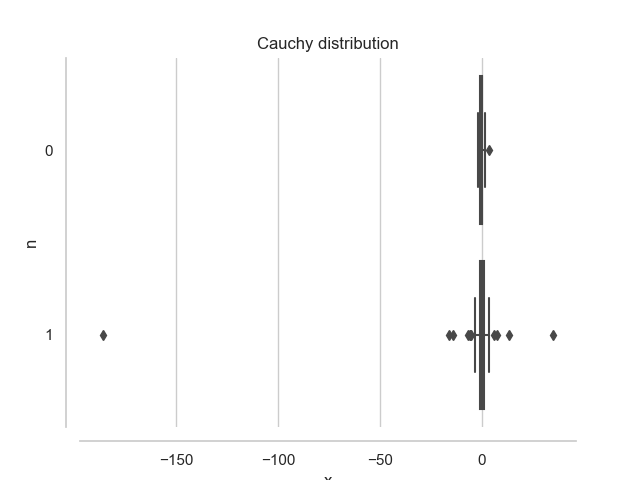
\includegraphics[scale=0.8]{figures/CauchyBoxplot.png}
        \caption{Распределение Коши}
        \label{fig:normal}
    \end{figure}
    
    \begin{figure}[H]
        \centering
        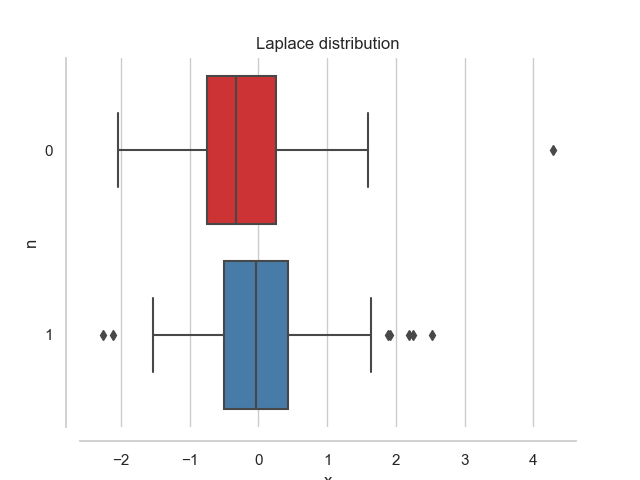
\includegraphics[scale=0.8]{figures/LaplaceBoxplot.png}
        \caption{Распределение Лапласа}
        \label{fig:normal}
    \end{figure}
    
     \begin{figure}[H]
        \centering
        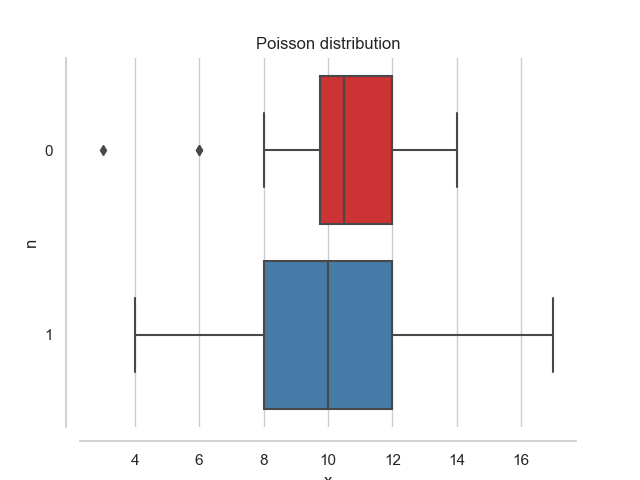
\includegraphics[scale=0.8]{figures/PoissonBoxplot.png}
        \caption{Распределение Пуассона}
        \label{fig:normal}
    \end{figure}
    
    \begin{figure}[H]
        \centering
        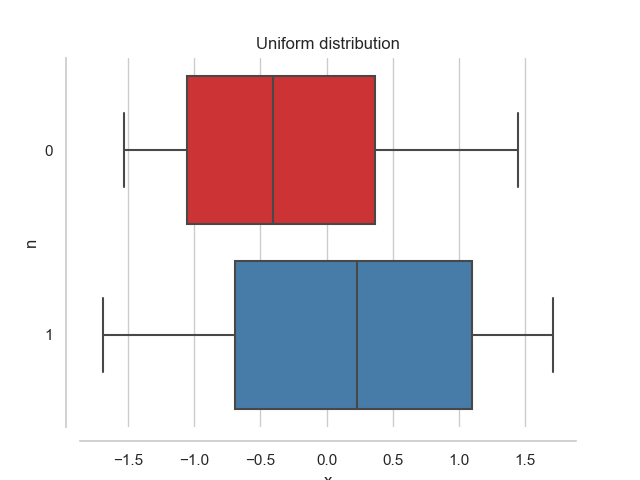
\includegraphics[scale=0.8]{figures/UniformBoxplot.png}
        \caption{Равномерное распределение}
        \label{fig:normal}
    \end{figure}
    
    \subsection{Доля выбросов}
    \begin{table}[H]
	\centering
	\begin{tabular}{|l|c|c|}
		\hline
		Выборка & Доля выбросов	\\\hline
		\hline
		Normal n = 20 & 0.0239 \\\hline
		Normal n = 100 & 0.0099 \\\hline
		Cauchy n = 20 & 0.1476 \\\hline
		Cauchy n = 100 & 0.1541 \\\hline
		Laplace n = 20 & 0.0771 \\\hline
		Laplace n = 100 & 0.065 \\\hline
		Poisson n = 20 & 0.022 \\\hline
		Poisson n = 100 & 0.0111 \\\hline
		Uniform n = 20 & 0.0026 \\\hline
		Uniform n = 100 & 0 \\\hline
	\end{tabular}
	\caption{Практическая доля выбросов}
    \end{table}
    
    \subsection{Теоретическая вероятность выбросов}
    
    \begin{table}[H]
	\centering
	\begin{tabular}{|l|c|c|c|c|c|}
		\hline
		Распределение & $Q_1^T$	& $Q_3^T$ & $X_1^T$ & $X_2^T$ & $P_B^T$\\\hline
		\hline
		Нормальное & -0.674 & 0.674 & -2.698 &  2.698 & 0.007\\\hline
		Коши & -1 & 1 & -4 & 4 & 0.156\\\hline
		Лапласа & -0.490 & 0.490 & -1.961 & 1.961 & 0.063\\\hline
		Пуассона & 8 & 12 & 2 & 18 & 0.008\\\hline
		Равномерное & -0.866 & 0.866 & -3.464 & 3.464 & 0\\\hline
	\end{tabular}
	\caption{Теоретическая вероятность выбросов}
    \end{table}
    
    \subsection{Эмпирическая функция распределения}
    
    \begin{figure}[H]
        \centering
        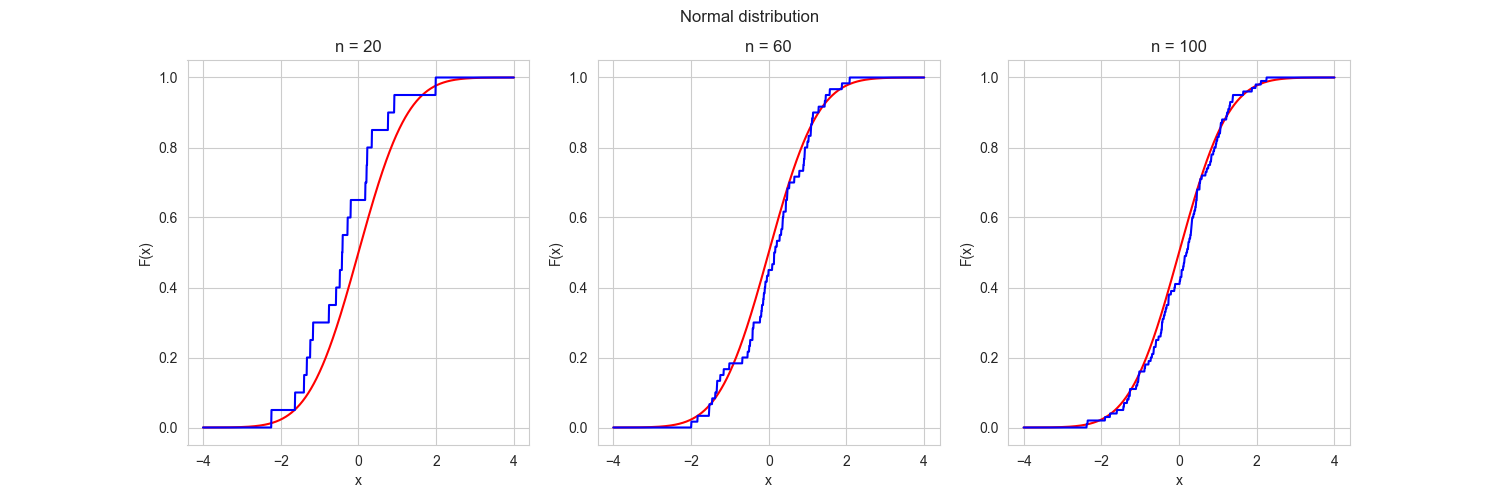
\includegraphics[scale=0.5]{figures/NormalEmpirical.png}
        \caption{Нормальное распределение}
        \label{fig:normal}
    \end{figure}
    
    \begin{figure}[H]
        \centering
        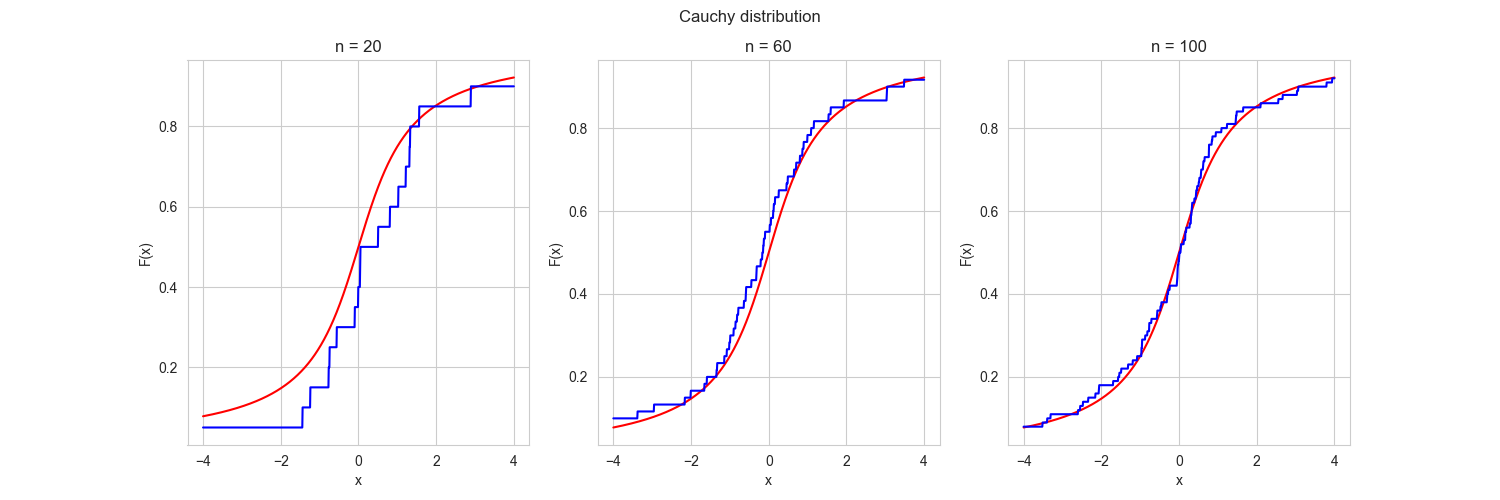
\includegraphics[scale=0.5]{figures/CauchyEmpirical.png}
        \caption{Распределение Коши}
        \label{fig:normal}
    \end{figure}
    
    \begin{figure}[H]
        \centering
        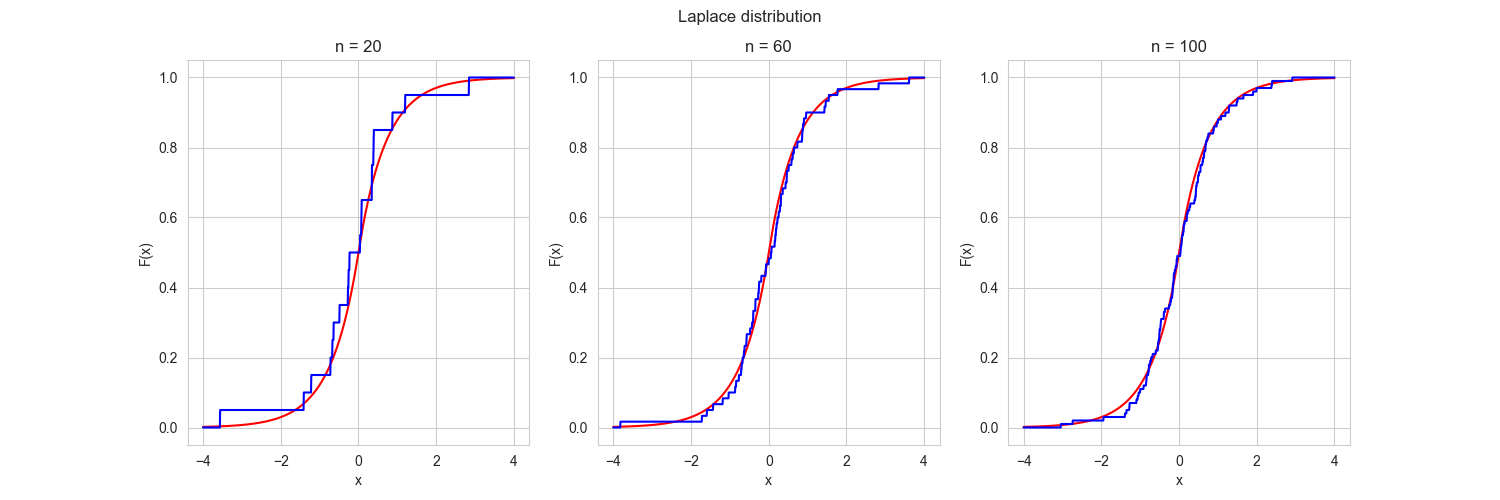
\includegraphics[scale=0.5]{figures/LaplaceEmpirical.png}
        \caption{Распределение Лапласа}
        \label{fig:normal}
    \end{figure}
    
     \begin{figure}[H]
        \centering
        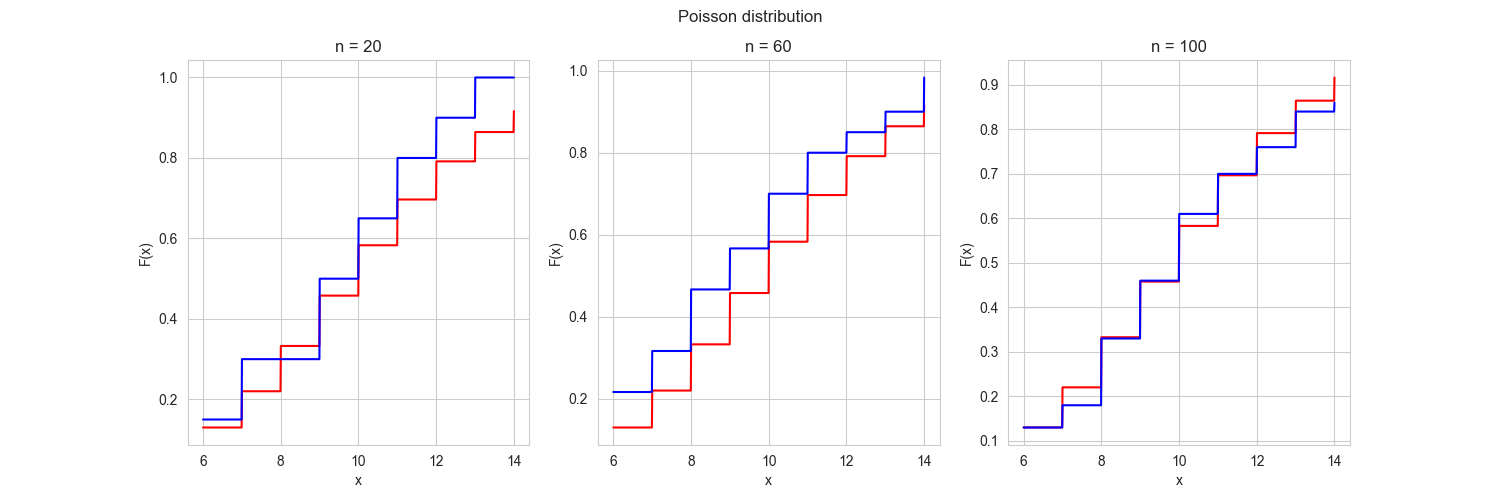
\includegraphics[scale=0.5]{figures/PoissonEmpirical.png}
        \caption{Распределение Пуассона}
        \label{fig:normal}
    \end{figure}
    
    \begin{figure}[H]
        \centering
        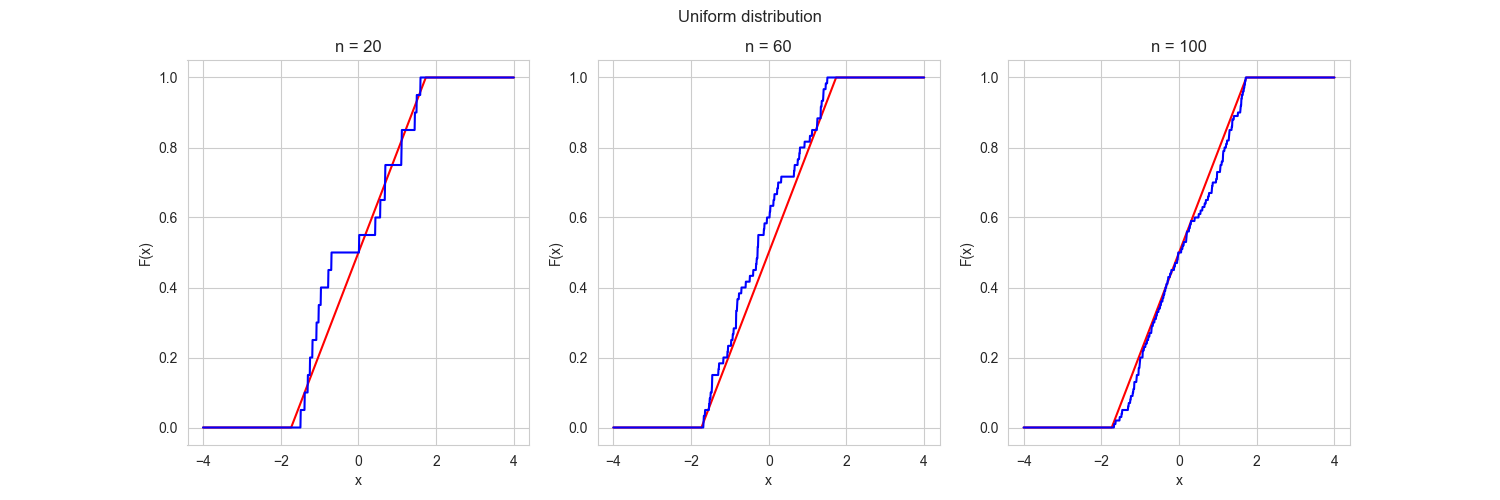
\includegraphics[scale=0.5]{figures/UniformEmpirical.png}
        \caption{Равномерное распределение}
        \label{fig:normal}
    \end{figure}
    
    \subsection{Ядерные оценки плотности распределения}
    
    \begin{figure}[H]
        \centering
        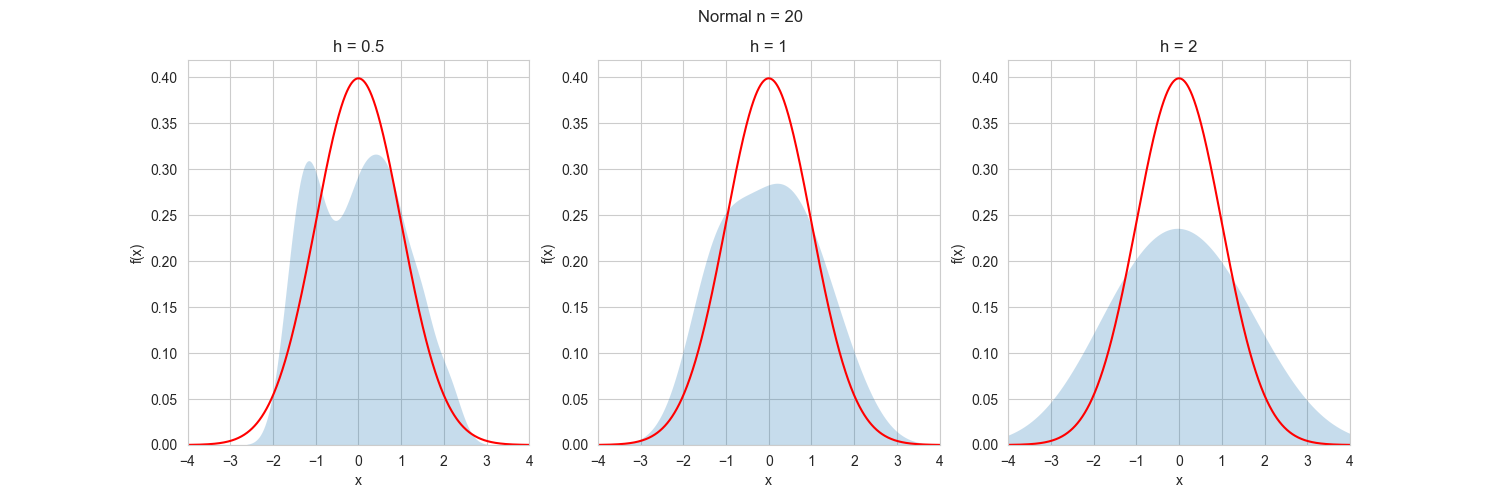
\includegraphics[scale=0.5]{figures/NormalNuclear20.png}
        \caption{Нормальное распределение, n = 20}
        \label{fig:normal}
    \end{figure}
    
    \begin{figure}[H]
        \centering
        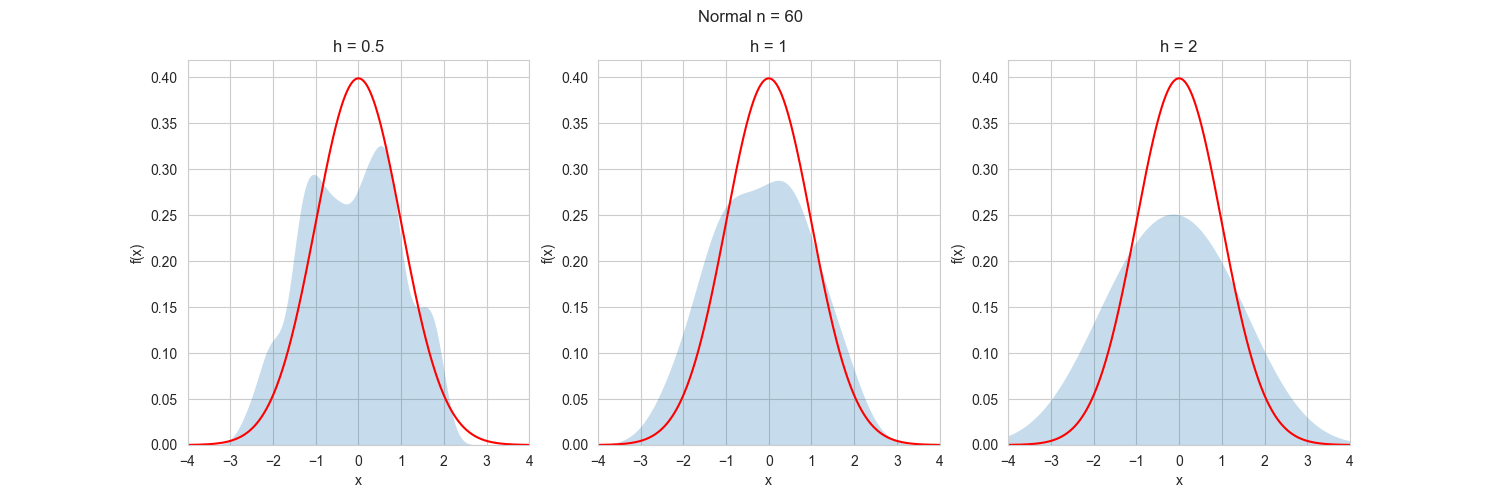
\includegraphics[scale=0.5]{figures/NormalNuclear60.png}
        \caption{Нормальное распределение, n = 60}
        \label{fig:normal}
    \end{figure}
    
    \begin{figure}[H]
        \centering
        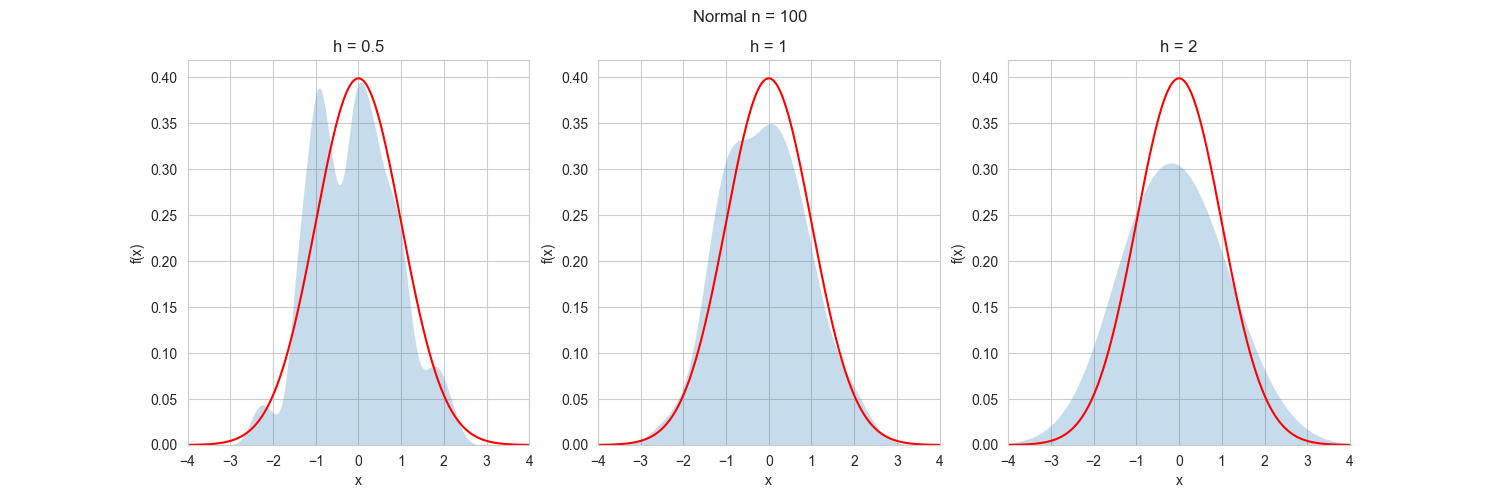
\includegraphics[scale=0.5]{figures/NormalNuclear100.png}
        \caption{Нормальное распределение, n = 100}
        \label{fig:normal}
    \end{figure}
    
    \begin{figure}[H]
        \centering
        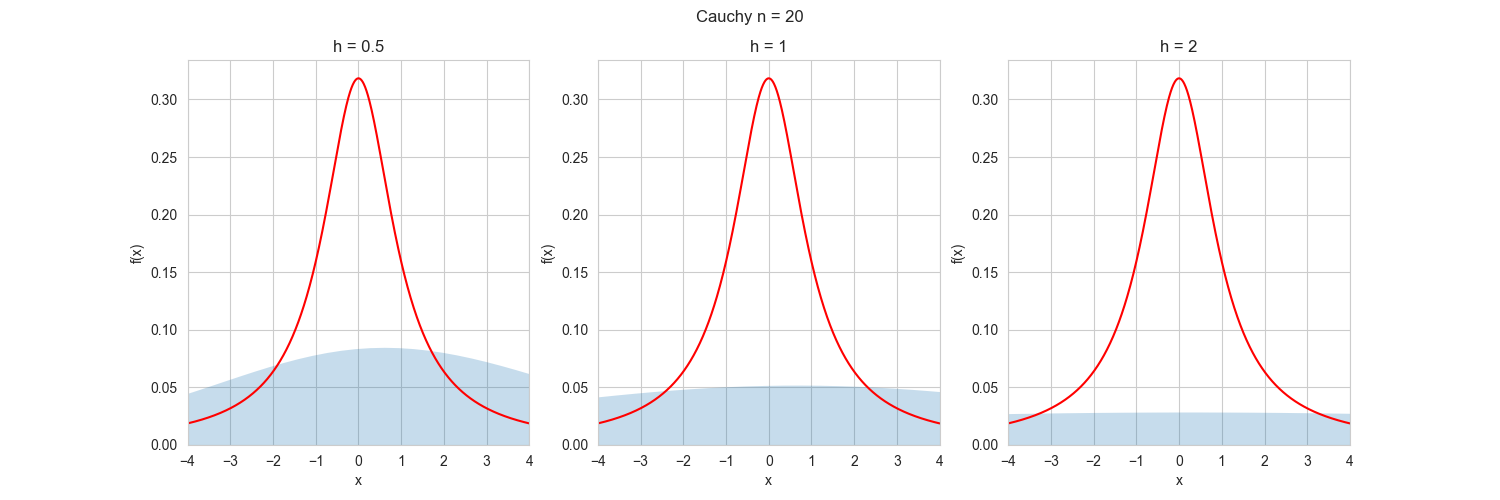
\includegraphics[scale=0.5]{figures/CauchyNuclear20.png}
        \caption{Распределение Коши, n = 20}
        \label{fig:normal}
    \end{figure}
    
    \begin{figure}[H]
        \centering
        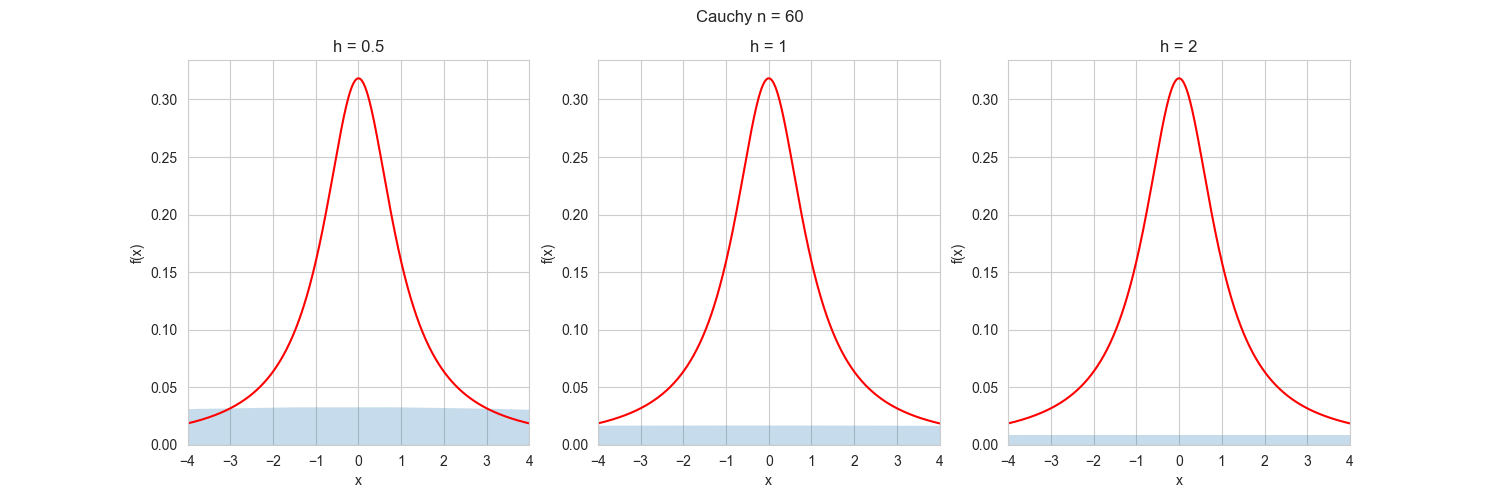
\includegraphics[scale=0.5]{figures/CauchyNuclear60.png}
        \caption{Распределение Коши, n = 60}
        \label{fig:normal}
    \end{figure}
    
    \begin{figure}[H]
        \centering
        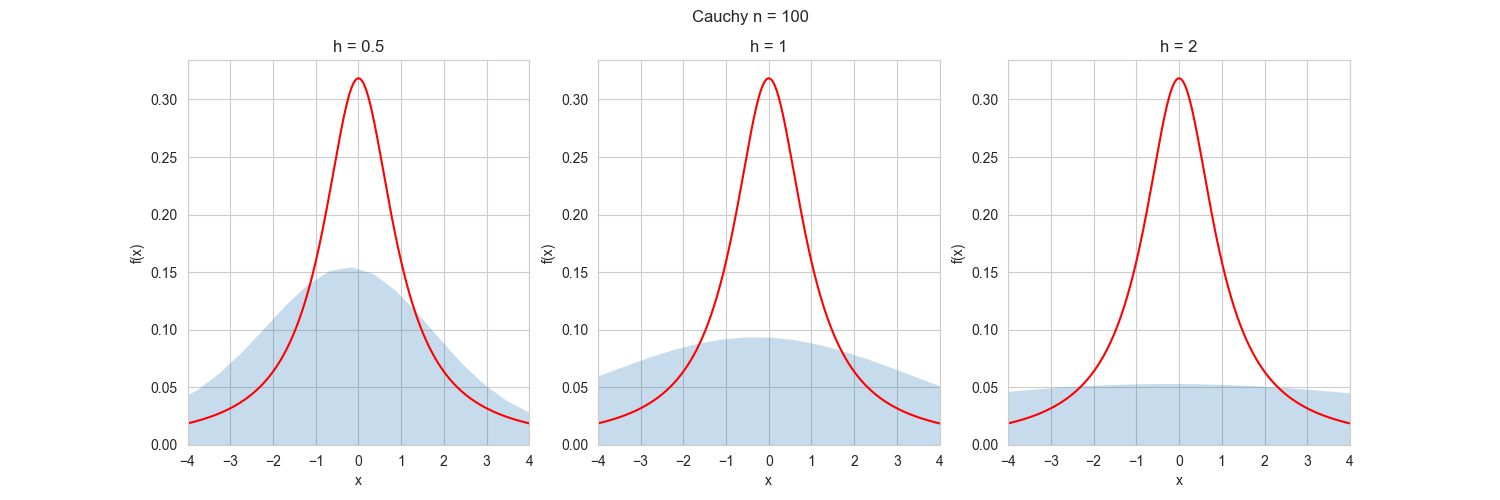
\includegraphics[scale=0.5]{figures/CauchyNuclear100.png}
        \caption{Распределение Коши, n = 100}
        \label{fig:normal}
    \end{figure}
    
    \begin{figure}[H]
        \centering
        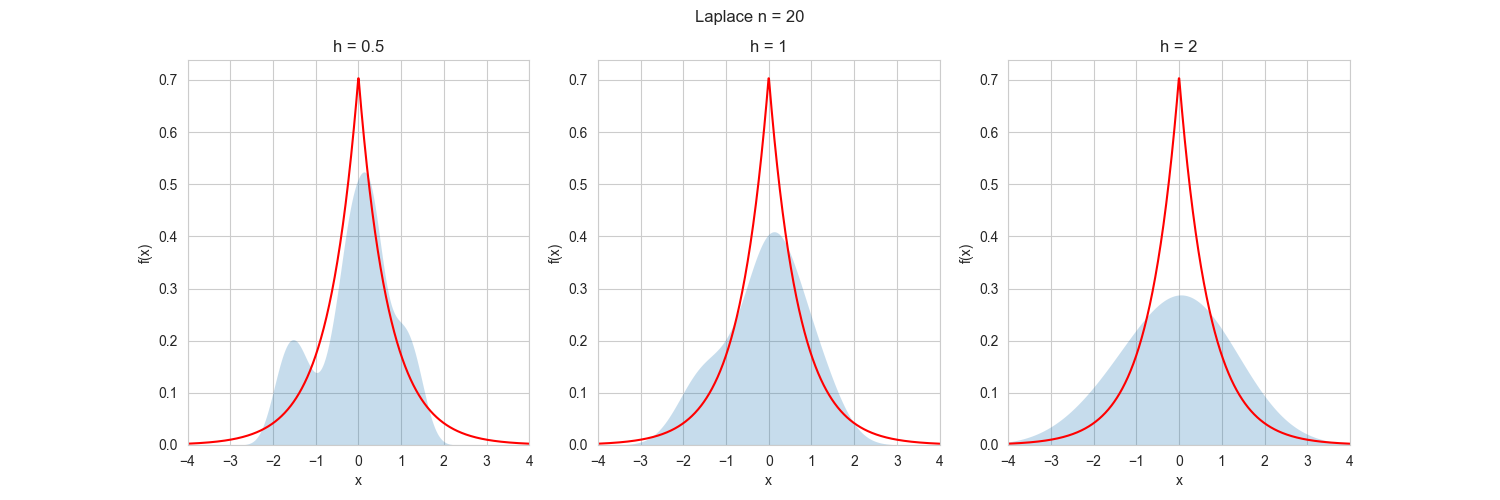
\includegraphics[scale=0.5]{figures/LaplaceNuclear20.png}
        \caption{Распределение Лапласа, n = 20}
        \label{fig:normal}
    \end{figure}
    
    \begin{figure}[H]
        \centering
        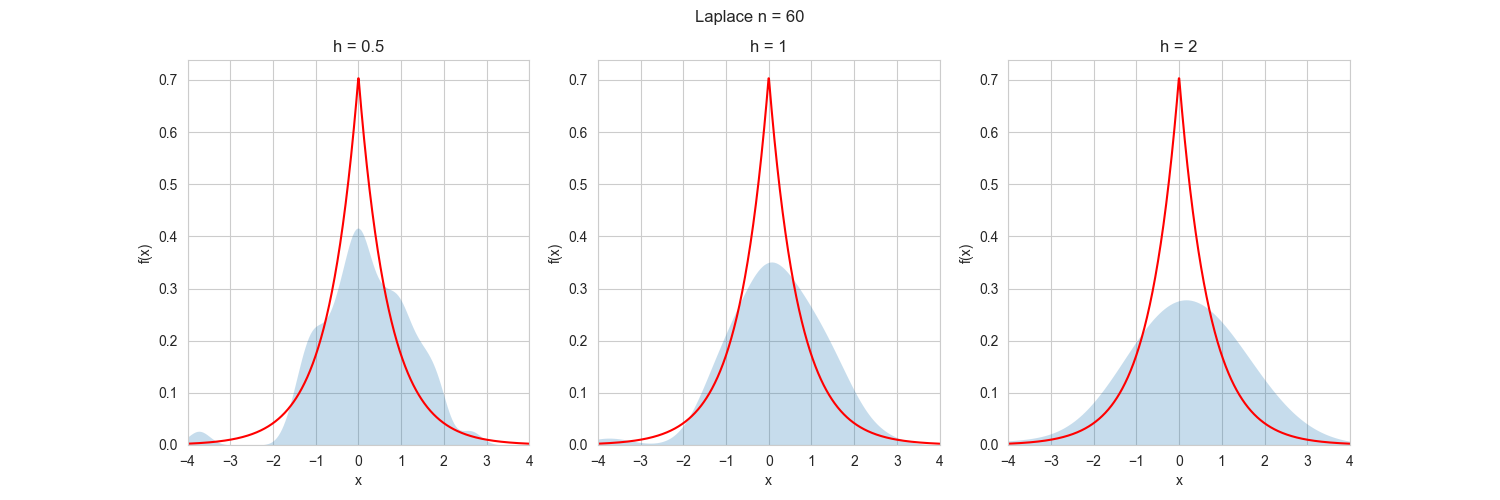
\includegraphics[scale=0.5]{figures/LaplaceNuclear60.png}
        \caption{Распределение Лапласа, n = 60}
        \label{fig:normal}
    \end{figure}
    
    \begin{figure}[H]
        \centering
        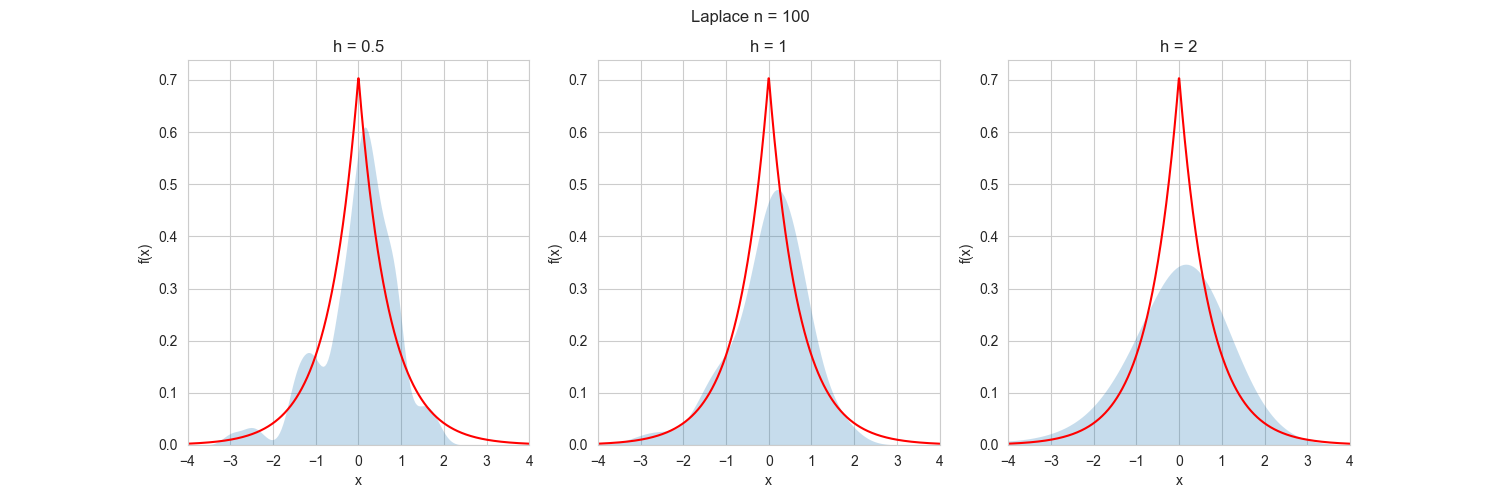
\includegraphics[scale=0.5]{figures/LaplaceNuclear100.png}
        \caption{Распределение Лапласа, n = 100}
        \label{fig:normal}
    \end{figure}
    
    \begin{figure}[H]
        \centering
        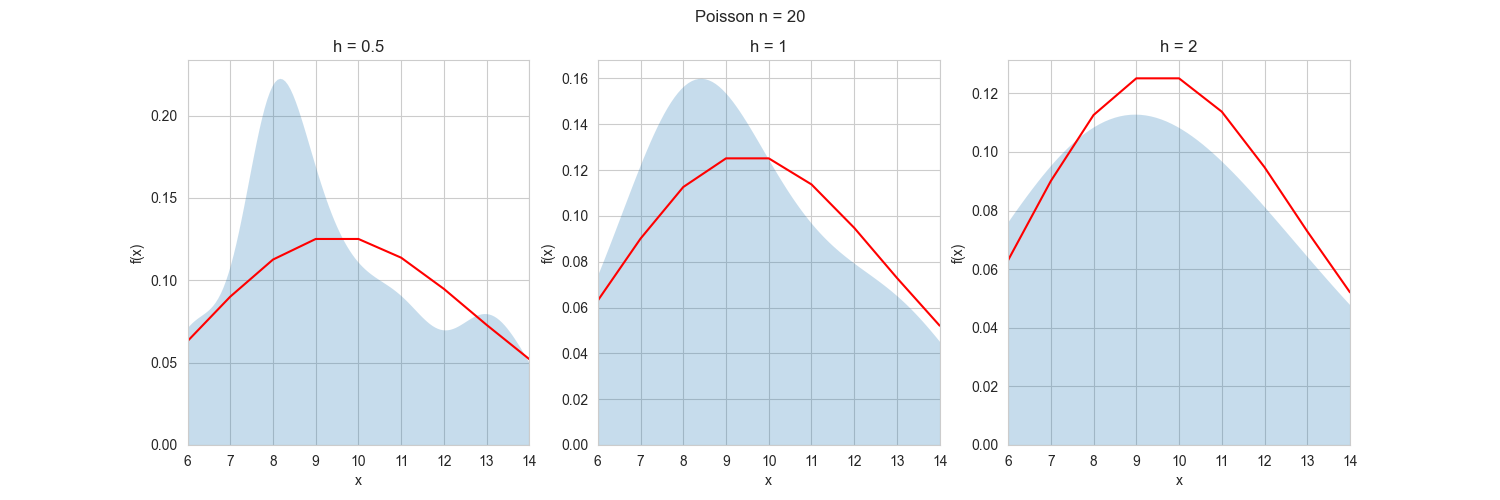
\includegraphics[scale=0.5]{figures/PoissonNuclear20.png}
        \caption{Распределение Пуассона, n = 20}
        \label{fig:normal}
    \end{figure}
    
    \begin{figure}[H]
        \centering
        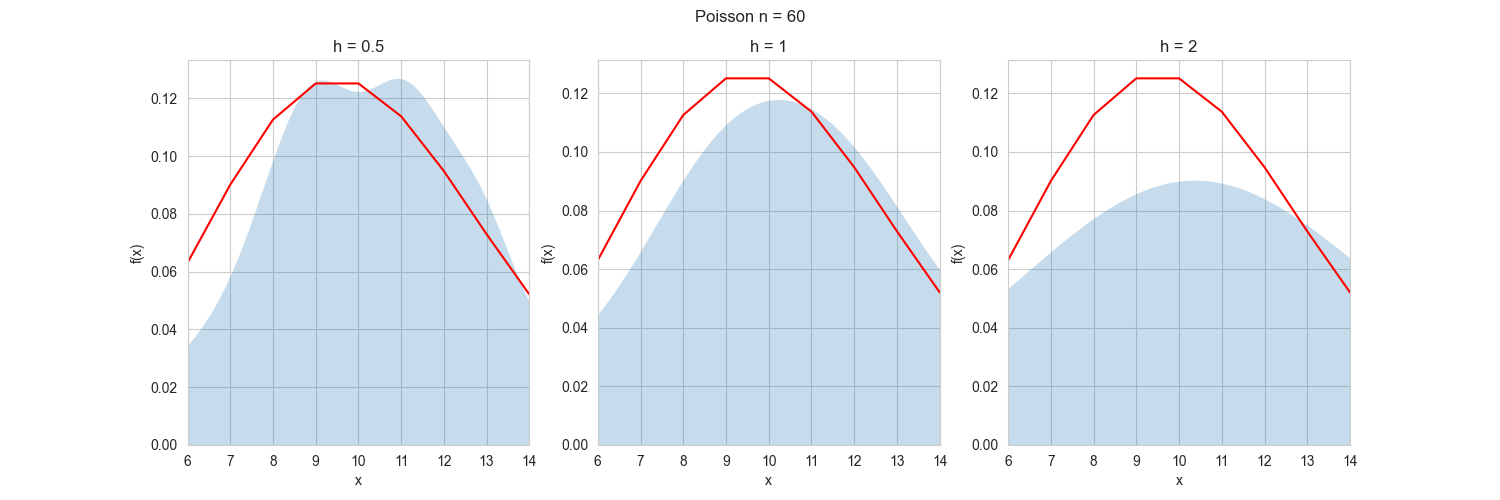
\includegraphics[scale=0.5]{figures/PoissonNuclear60.png}
        \caption{Распределение Пуассона, n = 60}
        \label{fig:normal}
    \end{figure}
    
    \begin{figure}[H]
        \centering
        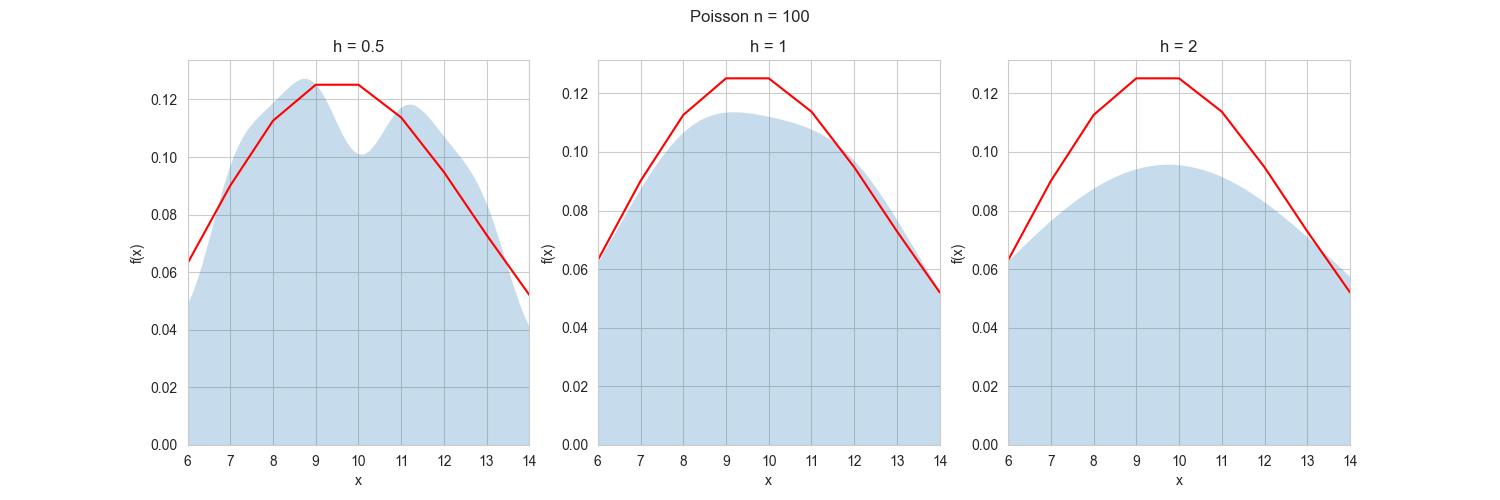
\includegraphics[scale=0.5]{figures/PoissonNuclear100.png}
        \caption{Распределение Пуассона, n = 100}
        \label{fig:normal}
    \end{figure}
    
    \begin{figure}[H]
        \centering
        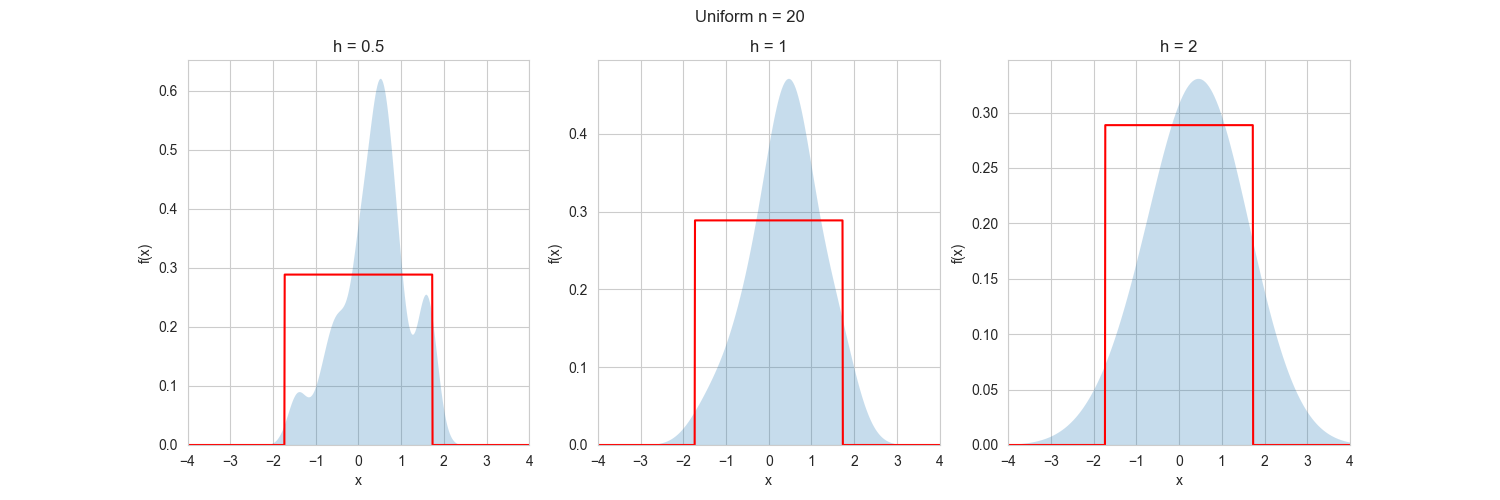
\includegraphics[scale=0.5]{figures/UniformNuclear20.png}
        \caption{Равномерное распределение, n = 20}
        \label{fig:normal}
    \end{figure}
    
    \begin{figure}[H]
        \centering
        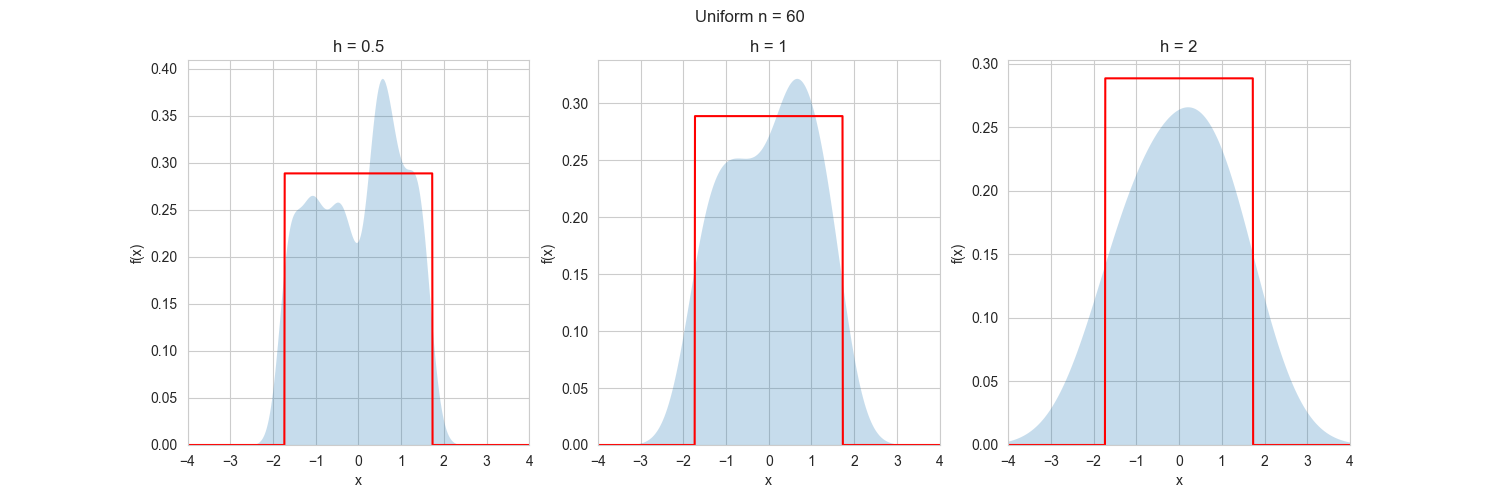
\includegraphics[scale=0.5]{figures/UniformNuclear60.png}
        \caption{Равномерное распределение, n = 60}
        \label{fig:normal}
    \end{figure}
    
    \begin{figure}[H]
        \centering
        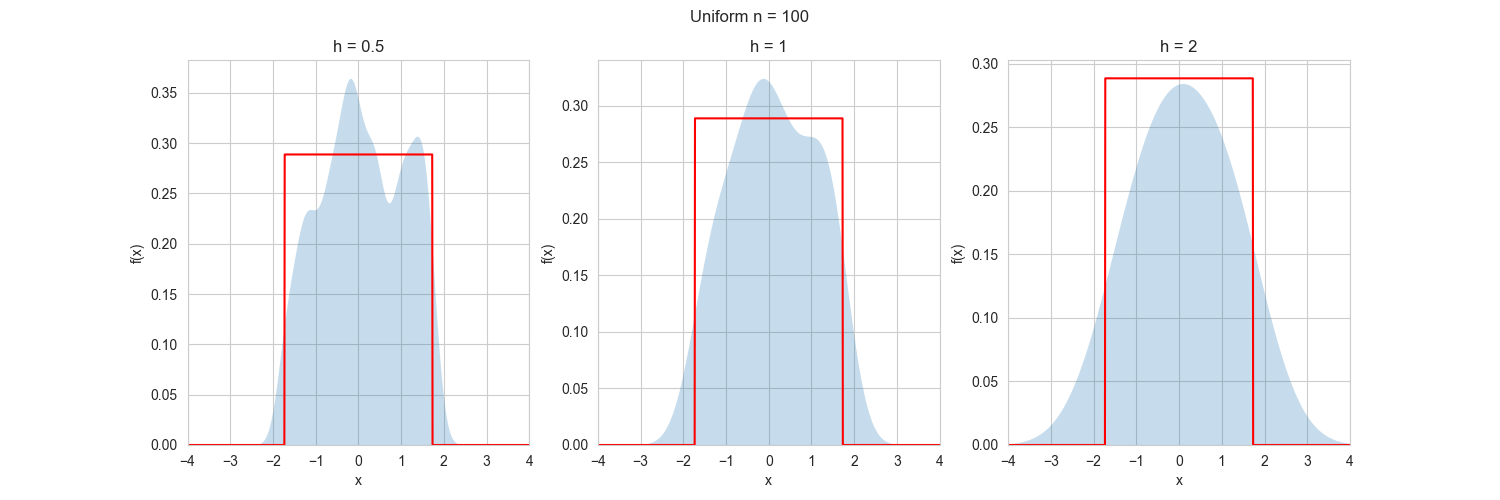
\includegraphics[scale=0.5]{figures/UniformNuclear100.png}
        \caption{Равномерное распределение, n = 100}
        \label{fig:normal}
    \end{figure}
\end{document}